\documentclass[letterpaper, 12pt]{article}

%%%%%%%%%%%%%%%%%%%%%%%%%%%%%
% DEFINITIONS
% Change those informations
% If you need umlauts you have to escape them, e.g. for an ü you have to write \"u
\gdef\mytitle{Laborprotokoll}
\gdef\mythema{DezSys09 - Web Services in Java}

\gdef\mysubject{Systemtechnik}
\gdef\mycourse{5BHIT 2015/16, Gruppe B}
\gdef\myauthor{Michael Weinberger}

\gdef\myversion{1.0}
\gdef\mybegin{11. M\"arz 2016}
\gdef\myfinish{\today}

\gdef\mygrade{Note:}
\gdef\myteacher{Betreuer: Borko}
%
%%%%%%%%%%%%%%%%%%%%%%%%%%%%%

\input special/preamble.tex

\let\tempsection\section
\renewcommand\section[1]{\vspace{-0.3cm}\tempsection{#1}\vspace{-0.3cm}}
\WithSuffix\newcommand\section*[1]{\tempsection*{#1}}

\let\tempsubsection\subsection
\renewcommand\subsection[1]{\vspace{0cm}\tempsubsection{#1}\vspace{0cm}}

\let\tempsubsubsection\subsubsection
\renewcommand\subsubsection[1]{\vspace{0cm}\tempsubsubsection{#1}\vspace{0cm}}

\linespread{0.94}

\lhead{\mysubject}
\chead{}
\rhead{\bfseries\mythema}
\lfoot{\mycourse}
\cfoot{\thepage}
% Creative Commons license BY
% http://creativecommons.org/licenses/?lang=de
\rfoot{\ccby\hspace{2mm}\myauthor}
\renewcommand{\headrulewidth}{0.4pt}
\renewcommand{\footrulewidth}{0.4pt}

\begin{document}
\parindent 0pt
\parskip 6pt

\pagenumbering{Roman} 
%!TEX root=../laborprotokoll.tex

\begin{titlepage}

	\begin{figure}[!h]
		\begin{flushright}
			
\includegraphics[width=0.3\linewidth]{images/jdIT_tgm.png}
		\end{flushright}
	\end{figure}

	\vspace{2.5cm} 

	{\begin{center} \bfseries\huge
			\rule{17.5cm}{0.1mm}  
			\\[5mm]
			\mytitle\\[5mm]
			\mythema\\
			\rule{17.5cm}{0.1mm}  
	\end{center}}

	{\begin{flushright} \bfseries\Large
			\vspace{2cm}
			\mysubject\\
			\mycourse\\[10mm]
			\myauthor\\[10mm]
	\end{flushright}}

	{\begin{table}[!h] \bfseries\normalsize
		\begin{tabularx}{\textwidth}{lXr @{\hspace{0mm}}}
			&& Version \myversion\\
			\mygrade && Begonnen am \mybegin\\
			\myteacher && Beendet am \myfinish\\
		\end{tabularx}
	\end{table}}

\end{titlepage}


\clearpage
\thispagestyle{empty}
\tableofcontents

\newpage
\pagenumbering{arabic}
\pagestyle{fancy}

%\vspace{-0.5cm}
\section{Einführung}
Diese Übung zeigt die Anwendung von mobilen Diensten in Java.

\subsection{Ziele}
Das Ziel dieser Übung ist eine Webanbindung zur Benutzeranmeldung in Java umzusetzen. Dabei soll sich ein Benutzer registrieren und am System anmelden können. \\
Die Kommunikation zwischen Client und Service soll mit Hilfe von JAX-RS (Gruppe 1+2) umgesetzt werden.

\subsection{Voraussetzungen}
\begin{itemize}
	\item Grundlagen Java und Java EE
	\item Verständnis über relationale Datenbanken und dessen Anbindung mittels JDBC oder ORM-Frameworks
	\item Verständnis von Restful Webservices
\end{itemize}

\subsection{Aufgabenstellung}
Es ist ein Webservice mit Java zu implementieren, welches eine einfache Benutzerverwaltung implementiert. Dabei soll die Webapplikation mit den Endpunkten /register und /login erreichbar sein. \\ \\
\textit{Registrierung} \\
Diese soll mit einem Namen, einer eMail-Adresse als BenutzerID und einem Passwort erfolgen. Dabei soll noch auf keine besonderen Sicherheitsmerkmale Wert gelegt werden. Bei einer erfolgreichen Registrierung (alle Elemente entsprechend eingegeben) wird der Benutzer in eine Datebanktabelle abgelegt. \\ \\
\textit{Login} \\
Der Benutzer soll sich mit seiner ID und seinem Passwort entsprechend authentifizieren können. Bei einem erfolgreichen Login soll eine einfache Willkommensnachricht angezeigt werden. \\ \\
Die erfolgreiche Implementierung soll mit entsprechenden Testfällen (Acceptance-Tests bez. aller funktionaler Anforderungen mittels JUnit) dokumentiert werden. Es muss noch keine grafische Oberfläche implementiert werden! Verwenden Sie auf jeden Fall ein gängiges Build-Management-Tool (z.B. Maven). Dabei ist zu beachten, dass ein einfaches Deployment möglich ist (auch Datenbank mit z.B. file-based DBMS).
\cite{eins, zwei, drei, vier}

\newpage

\section{Durchführung}

Link zum Repo \cite{repo} \newline
Zur Umsetzung wurde das Spring-Framework verwendet, da es im Vergleich einfach zu verwenden und aufzusetzen ist, und einen integrierten Applikationsserver bietet. Die Verwendung von JAX-RS wurde in dieser Übung vorgeschrieben. Auf einen Hinweis durch den Professor wurde keine überbordene relationale Datenbank verwendet, sondern die dateibasierte und gut unterstützte H2-Datenbank. Als Buildmanagement-Tool wurde Maven verwendet. Es wurde eine Vielzahl an Quellen herangenommen, wie es empfohlen wurde. Ein in den Quellen verlinktes Tutorial ('Bootiful' Java EE Support in Spring Boot 1.2) wurde übernommen und an unsere Bedürfnisse angepasst. Ebenso wurde als Einarbeitung bestehender Code hergenommen und analysiert, um schnell einen besseren Einblick zu bekommen. Wichtige, noch nicht vorhandene Teile waren etwa die RESTful Endpoints für Login und Register, auch die Datenbankanbindung musste angepasst werden. \cite{booti, spring, jaxrs, maven, hzwei, plugin, repoeins, repozwei}

\section{Akzeptanzkriterien}
\subsection{Registrierung}
Die Funktionalitätsüberprüfung nach den vorgeschriebenen Anforderungen wurde mithilfe des Firefox-Plugins 'HttpRequester' durchgeführt. \cite{plugin}
\subsubsection{Erfolgreiche Registrierung}
\begin{figure}[h]
	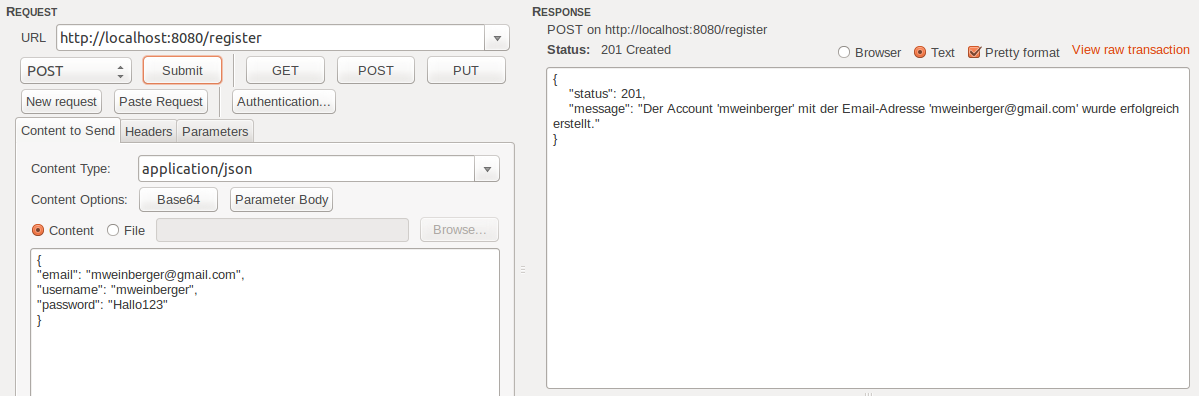
\includegraphics[width=1\textwidth]{images/reg_erf}
	\caption{Wenn alle Parameter gegeben sind, wird der Account erstellt.}
\end{figure} 
\clearpage

\subsubsection{Fehlende Parameter}
\begin{figure}[h]
	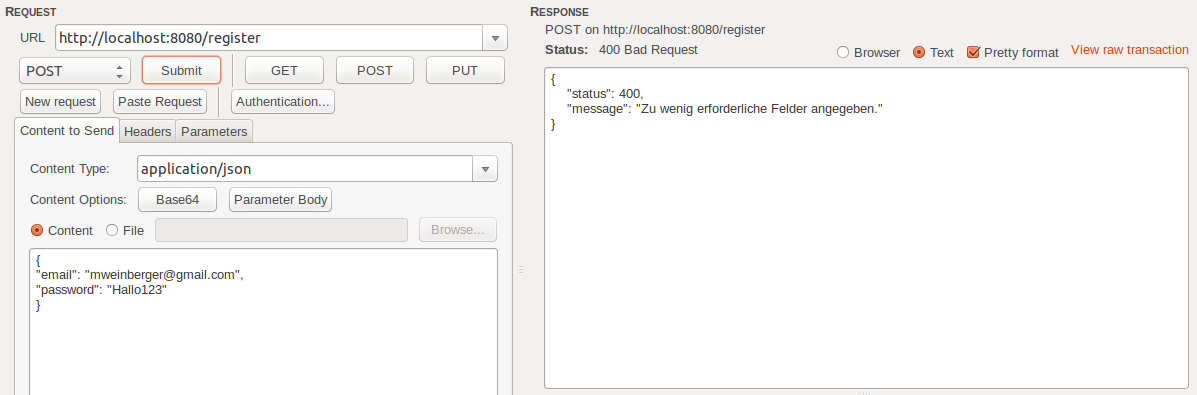
\includegraphics[width=1\textwidth]{images/reg_less}
	\caption{Wenn ein oder mehrere der erforderlichen Parameter fehlen, wird der Account nicht erstellt, und der Benutzer wird informiert.}
\end{figure}

\subsubsection{Bereits existenter Benutzer}
\begin{figure}[h]
	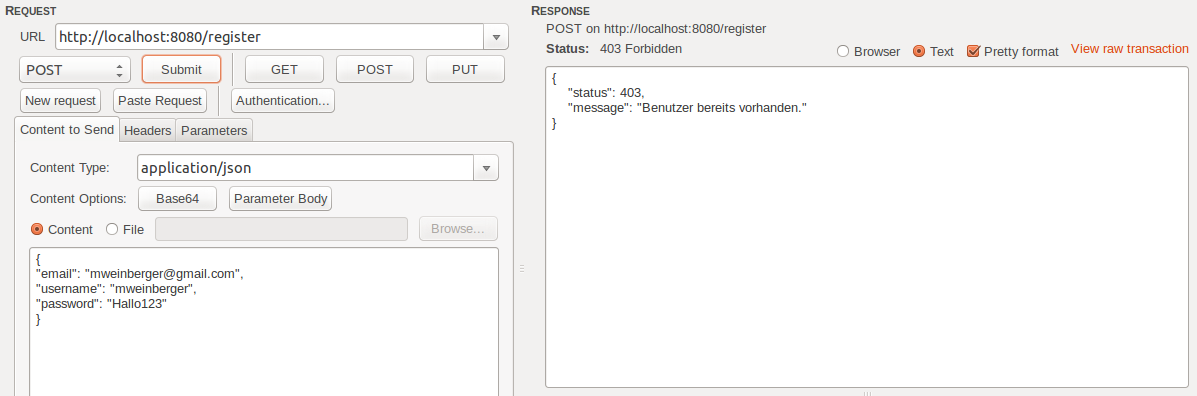
\includegraphics[width=1\textwidth]{images/reg_vorh}
	\caption{Ist der Benutzer bereits in der Datenbank vorhanden wird kein Account angelegt, und der Benutzer wird informiert.}
\end{figure}
\clearpage

\subsection{Login}
\subsubsection{Erfolgreicher Login}
\begin{figure}[h]
	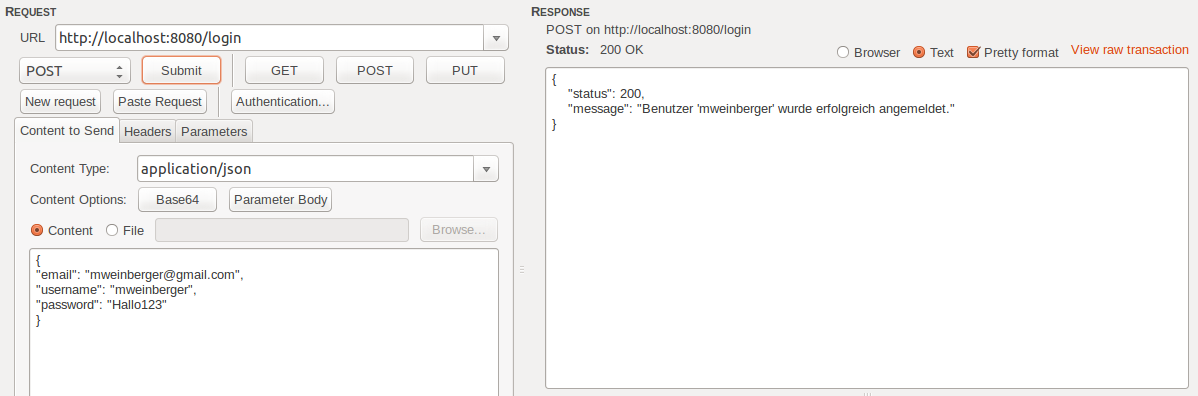
\includegraphics[width=1\textwidth]{images/login_erf}
	\caption{Wenn alle Parameter gegeben sind und der User in der Datenbank gefunden wird, ist der Benutzer erfolgreich angemeldet.}
\end{figure}

\subsubsection{Fehlende Parameter}
\begin{figure}[h]
	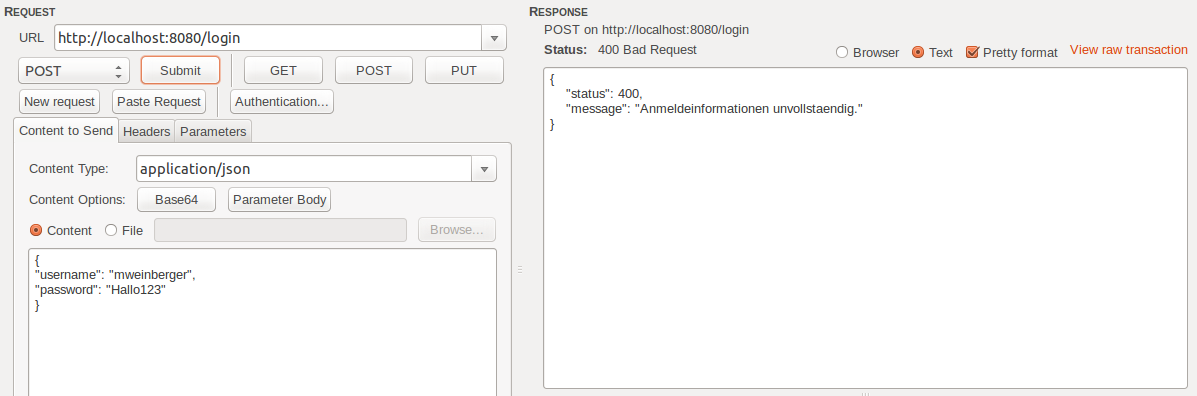
\includegraphics[width=1\textwidth]{images/login_unv}
	\caption{Wenn nicht alle Parameter gegeben sind, wird der Benutzer darauf hingewiesen.}
\end{figure}
\clearpage

\subsubsection{Benutzer nicht vorhanden}
\begin{figure}[h]
	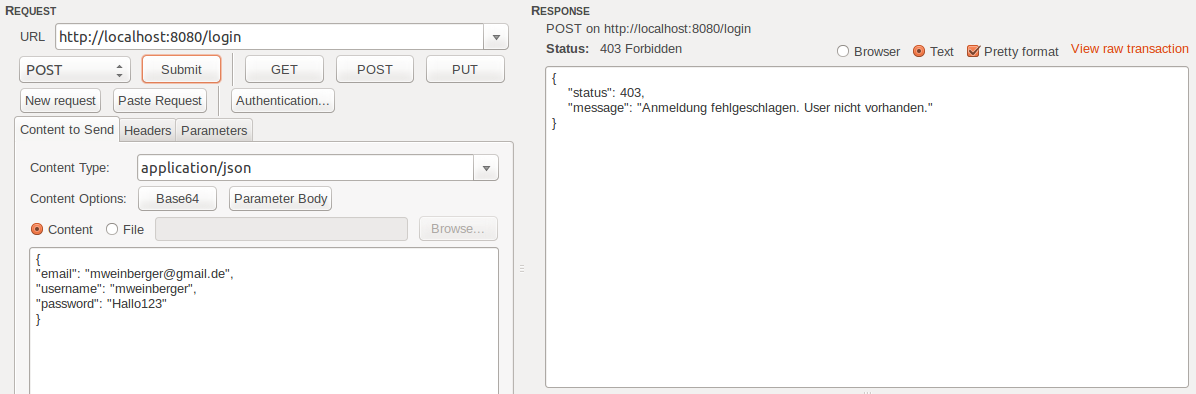
\includegraphics[width=1\textwidth]{images/login_fehl}
	\caption{Wenn der User nicht in der Datenbank gefunden wird, erhält der Benutzer die dazugehörige Fehlermeldung.}
\end{figure}

\subsection{Fazit}
Es gab anfängliche Probleme bei der Bereitstellung der Umgebung, aber ein Blick auf bestehende Lösungen konnte hier helfen. Fehlermeldungen zum Deployment konnten mit 5 Minuten Internetrecherche geklärt werden. Der Gesamtzeitaufwand dieser Aufgabe beträgt etwas mehr als 6 Stunden.

\newpage

\bibliographystyle{unsrt}
\bibliography{DezSys09_Weinb_5BHIT}
\clearpage
\listoffigures

\end{document}
